\ifx\inkludert\undefined
\documentclass[norsk,a4paper,twocolumn,oneside]{memoir}

\usepackage[utf8]{inputenc}
\usepackage{babel}
\usepackage{amsmath,amssymb,amsthm}
\usepackage[total={17cm,27cm}]{geometry}
\usepackage[table]{xcolor}
%\usepackage{tabularx}
\usepackage{systeme}
%\usepackage{hyperref}
%\usepackage{enumerate}

%\usepackage{sectsty}
\setsecheadstyle{\bfseries\large}
%\subsectionfont{\bf\normalsize}

\usepackage{tikz}
\usetikzlibrary{arrows.meta}

\newcommand{\defterm}[1]{\emph{#1}}

\newcommand{\N}{\mathbb{N}}
\newcommand{\Z}{\mathbb{Z}}
\newcommand{\Q}{\mathbb{Q}}
\newcommand{\R}{\mathbb{R}}

\newcommand{\abs}[1]{|#1|}

\newcommand{\roweq}{\sim}
\DeclareMathOperator{\Span}{Span}

\newcommand{\V}[1]{\mathbf{#1}}
\newcommand{\vv}[2]{\begin{bmatrix} #1 \\ #2 \end{bmatrix}}
\newcommand{\vvv}[3]{\begin{bmatrix} #1 \\ #2 \\ #3 \end{bmatrix}}
\newcommand{\vvvv}[4]{\begin{bmatrix} #1 \\ #2 \\ #3 \\ #4 \end{bmatrix}}
\newcommand{\vn}[2]{\vvvv{#1_1}{#1_2}{\vdots}{#1_#2}}

\newenvironment{amatrix}[1]{% "augmented matrix"
  \left[\begin{array}{*{#1}{c}|c}
}{%
  \end{array}\right]
}

% \newcounter{notatnr}
% \newcommand{\notatnr}[2]
% {\setcounter{notatnr}{#1}%
%  \setcounter{page}{#2}%
% }

\newtheorem{thm}{Teorem}[chapter]
\newtheorem*{thm-nn}{Teorem}
\newtheorem{cor}[thm]{Korollar}
\newtheorem{lem}[thm]{Lemma}
\newtheorem{prop}[thm]{Proposisjon}
\theoremstyle{definition}
\newtheorem{exx}[thm]{Eksempel}
\newtheorem*{defnx}{Definisjon}
\newtheorem*{oppg}{Oppgave}
\newtheorem*{merkx}{Merk}
\newtheorem*{spmx}{Spørsmål}

\newenvironment{defn}
  {\pushQED{\qed}\renewcommand{\qedsymbol}{$\triangle$}\defnx}
  {\popQED\enddefnx}
\newenvironment{ex}
  {\pushQED{\qed}\renewcommand{\qedsymbol}{$\triangle$}\exx}
  {\popQED\endexx}
\newenvironment{merk}
  {\pushQED{\qed}\renewcommand{\qedsymbol}{$\triangle$}\merkx}
  {\popQED\endmerkx}
\newenvironment{spm}
  {\pushQED{\qed}\renewcommand{\qedsymbol}{$\triangle$}\spmx}
  {\popQED\endspmx}

\setlength{\columnsep}{26pt}

\newcommand{\Tittel}[2]{%
\twocolumn[
\begin{center}
\Large
\begin{tabularx}{\textwidth}{cXr}
\cellcolor{black}\color{white}%
\bf {#1} &
#2
\hfill &
\footnotesize TMA4110 høsten 2018
\\ \hline
\end{tabularx}
\end{center}
]}

\newcommand{\tittel}[1]{\Tittel{\arabic{notatnr}}{#1}}

\newcommand{\linje}{%
\begin{center}
\rule{.8\linewidth}{0.4pt}
\end{center}
}


\newcommand{\chapternumber}{}

\makechapterstyle{tma4110}{%
 \renewcommand*{\chapterheadstart}{}
 \renewcommand*{\printchaptername}{}
 \renewcommand*{\chapternamenum}{}
 \renewcommand*{\printchapternum}{\renewcommand{\chapternumber}{\thechapter}}
 \renewcommand*{\afterchapternum}{}
 \renewcommand*{\printchapternonum}{\renewcommand{\chapternumber}{}}
 \renewcommand*{\printchaptertitle}[1]{
\LARGE
\begin{tabularx}{\textwidth}{cXr}
\cellcolor{black}\color{white}%
\textbf{\chapternumber} &
\textbf{##1}
\hfill &
%\footnotesize TMA4110 høsten 2018
\\ \hline
\end{tabularx}%
}
 \renewcommand*{\afterchaptertitle}{\par\nobreak\vskip \afterchapskip}
 % \newcommand{\chapnamefont}{\normalfont\huge\bfseries}
 % \newcommand{\chapnumfont}{\normalfont\huge\bfseries}
 % \newcommand{\chaptitlefont}{\normalfont\Huge\bfseries}
 \setlength{\beforechapskip}{0pt}
 \setlength{\midchapskip}{0pt}
 \setlength{\afterchapskip}{10pt}
}


\newcounter{oppgnr}[chapter]
\newcounter{punktnr}[oppgnr]
\newenvironment{oppgave}
 {\par\noindent\stepcounter{oppgnr}\textbf{{\arabic{oppgnr}}.}}
 {\par\bigskip}
\newenvironment{punkt}
 {\par\smallskip\noindent\stepcounter{punktnr}\textbf{\alph{punktnr})} }
 {\par}

\newcommand{\oppgaver}{\linje\section*{Oppgaver}}

\usepackage{xr}
\externaldocument{tma4110-2018h}
\newcommand{\kapittel}[2]{\setcounter{chapter}{#1}\addtocounter{chapter}{-1}\chapter{#2}}
\newcommand{\kapittelslutt}{\enddocument}
\begin{document}
\chapterstyle{tma4110}
\pagestyle{plain}
\fi


\kapittel{15}{Andre ordens lineære differensiallikninger}
\label{ch:andre-ordens-lineare-differensiallikninger}


\section*{Andre ordens differensiallikninger}
I matte 1 har du løst to typer differensiallikninger. Den ene er den første ordens lineære likningen
\[
y'+f(t)y=g(t)
\]
og den andre er den separable likningen
\[
y'=f(y)g(t).
\]
I dette avsnittet skal vi behandle lineære andreordens differensiallikninger med konstante koeffisienter:
\[
y''+a_1y'+a_0y=0
\]
Det er vanlig å kreve at $y \in \mathcal C^2$, altså at $y$ har to kontinuerlige deriverte. 
På denne måten kan man sikre at likningen faktisk gir mening. 
Det finnes mange situasjoner der dette kravet kan slakkes noe, 
men det er pensum i matte 4.  

Vi skal behandle den andre ordens differensiallikningen ved å skrive den om til et system 
%Dersom $f=0$, kalles likningen \defterm{homogen}. 
%Siden $L$ er en lineærtransformasjon, 
%kan vi umiddelbart dedusere at dersom to funksjoner er løser en homogen likning, 
%vil også lineærkombinasjoner av dem gjøre det. 
%Dette kalles \defterm{superposisjonsprinsippet}.






\section*{Hvor kommer andre ordens differensiallikninger fra?}
En kloss sklir friksjonsfritt p{\aa} underlaget, og er festet til veggen med en fj{\ae}r. Hookes fj{\ae}rlov sier at 
\begin{figure}[htbp]
  \begin{center}
	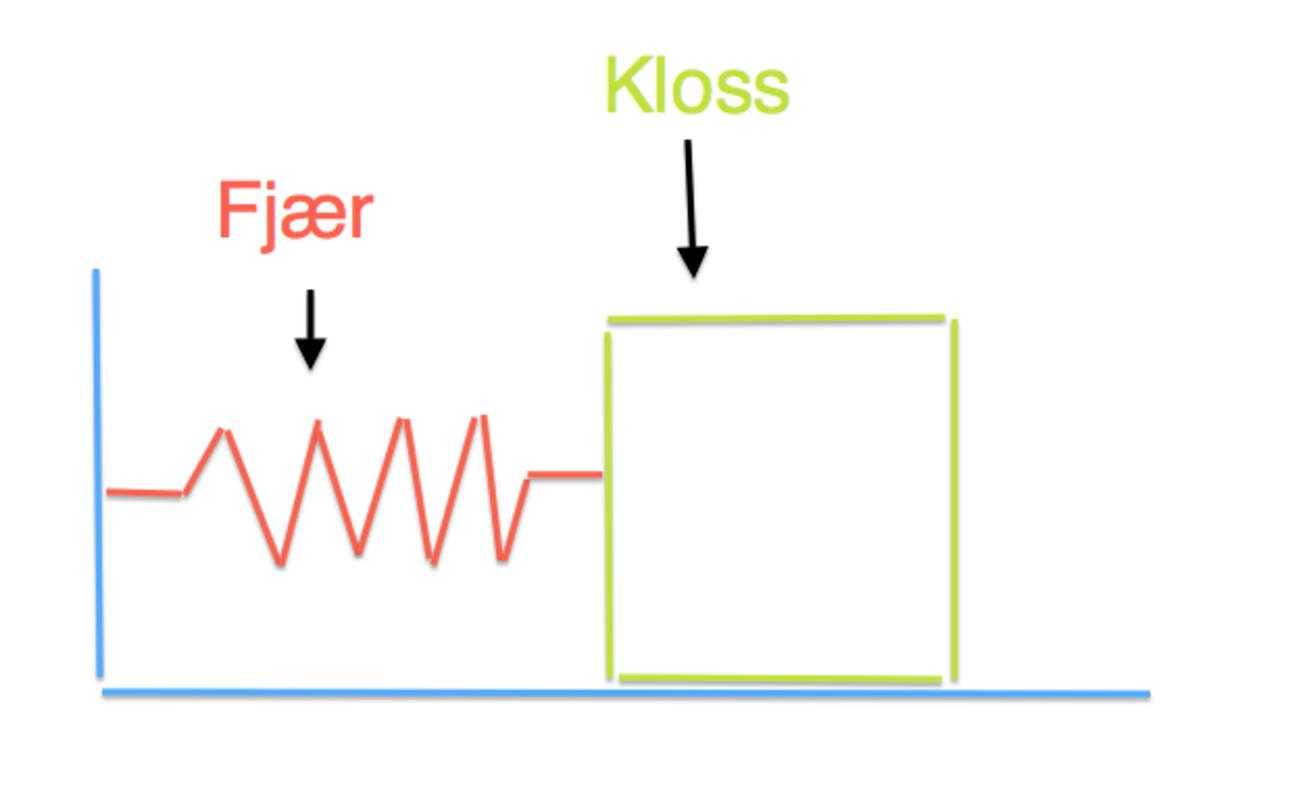
\includegraphics[scale=.35]{Hooke.pdf}
	\label{fig:Num1}
	\end{center}
\end{figure}
\[
F(x)=-kx,
\]
der $x$ er hvor langt fj{\ae}ren er strukket eller komprimert, 
$k$ er en konstant som avhenger av fj{\ae}rens stivhet, 
og $F(x)$ er kraften fra fj{\ae}ren p{\aa} klossen. 
Dersom $x(t)$ er klossens posisjon, er klossens akselerasjon gitt ved $x''(t)$,
og Newtons andre lov blir
\begin{equation*}
-kx=mx'',
\end{equation*}
der $m$ er klossens masse. Dette er en differensiallikning. Vi skriver vanligvis
\[
mx''+kx=0.
\]

Vi kan komplisere det litt til. La oss innf{\o}re luftmotstand. Luftmotstand avhenger kvadratisk av farten:
\begin{equation*}
F(x')=b(x')^{2};
\end{equation*}
der $b$ er en proporsjonalitetskonstant som sier noe om luftmotstanden. 
Den totale kraften blir
\begin{equation*}
F(x,x')=-kx+b(x')^{2},
\end{equation*}
slik at Newtons andre lov gir
\begin{equation*}
mx''-b(x')^{2} +kx=0.
\end{equation*}
Denne likningen har et problematisk ledd, $b(x')^{2}$. Men vi kan gjøre en forenkling. 
Dersom klossen ligger i en tyktflytende væske, blir motstanden proporsjonal med farten istedet for kvadratet av farten, 
og vi får likningen
\begin{equation*}
mx''-cx' +kx=0,
\end{equation*}
som er mye enklere å løse.



N{\aa} skal vi komplisere det enda litt. La klossen henge fra taket.
\begin{figure}[htbp]
  \begin{center}
	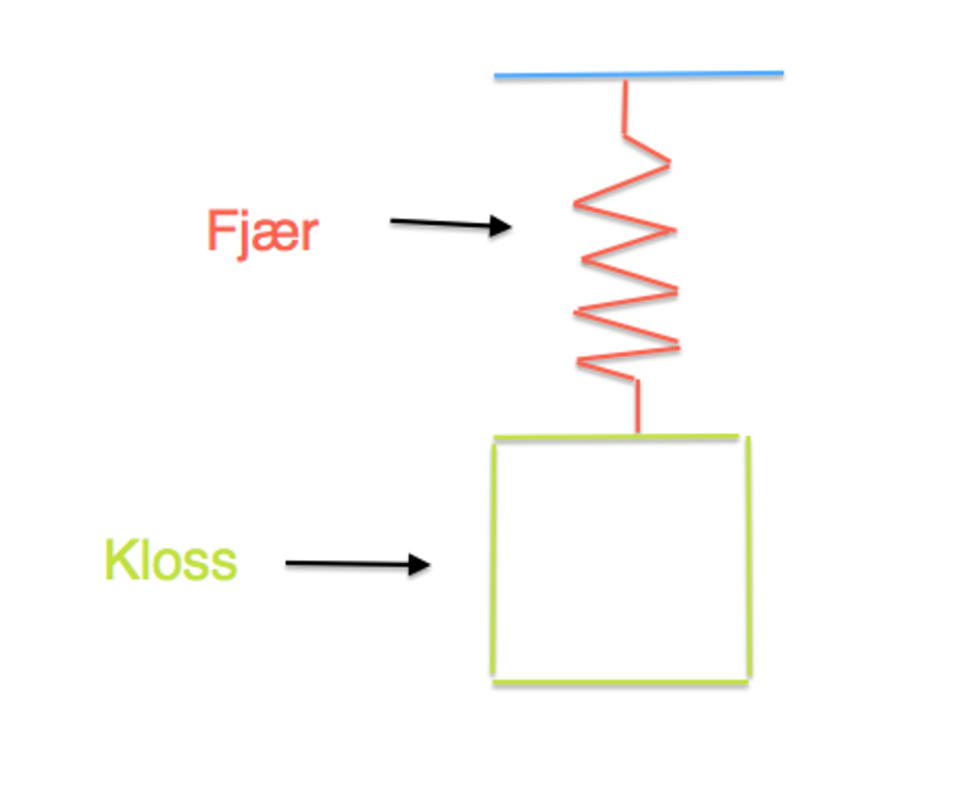
\includegraphics[scale=.4]{Hooke_2.pdf}
	\label{fig:Num1}
	\end{center}
\end{figure}
I tillegg til fj{\ae}rkraften og luftmotstanden, vil n{\aa} ogs{\aa} gravitasjonen p{\aa}virke bevegelsen. Gravitasjonskraften er en konstant kraft $mg$ nedover. Den totale kraften
er
\begin{equation*}
F(x,x')=-kx+bx'-mg,
\end{equation*}
og Newtons andre lov gir differensiallikningen
\begin{equation*}
mx''-bx' +kx=mg.
\end{equation*}





\section*{Omskrivning fra andre ordens likning til første ordens system}
En vanlig m{\aa}te {\aa} st{\o}te p{\aa} ligningssystemer p{\aa}, er dersom man omformer ligninger av h{\o}yere orden til f{\o}rste ordens systemer. Her er et eksempel. La 
\begin{equation*}
y''=-\sin y
\end{equation*}
Dette er en andre ordens differensialligning som beskriver bevegelsen til en pendel som dingler friksjonsfritt fra et opphengspunkt. N{\aa}r den henger rett ned, er $y=0$. Hvis vi
definerer
\begin{equation*}
y_{1}=y \quad \text{og} \quad y_{2}=y_{1}'
\end{equation*}
kan vi erstatte ligningen med det ekvivalente f{\o}rste ordens systemet
\begin{equation*}
y_{1}'=y_{2}
\end{equation*}
\begin{equation*}
y_{2}'=-\sin y_{1}.
\end{equation*}
Dette kan vi alltid gj{\o}re.


\section*{Løsningsteknikk for homogene ligninger}
Ligningen
\begin{equation*}
y'' +by' + cy=0
\end{equation*}
kalles en line{\ae}r, homogen \textbf{differensialligning} av andre orden.
For {\aa} l{\o}se ligningen, m{\aa} vi vite en ting, nemlig at l{\o}sningen er $y=e^{\lambda x}$. 
Det er ingenting {\aa} forst{\aa} med det, man m{\aa} bare \textbf{akseptere} det. 
For {\aa} finne $\lambda $, setter vi $y=e^{\lambda x}$ inn i ligningen:
\begin{equation*}
\lambda ^{2}e^{\lambda x} +b\lambda e^{\lambda x} + ce^{\lambda x}=0.
\end{equation*}
Vi trekker ut $e^{\lambda x}$
\begin{equation*}
(\lambda ^{2} +b\lambda  + c)e^{\lambda x}=0.
\end{equation*}
og siden $e^{kx}\neq 0$, m{\aa} vi ha
\begin{equation*}
\lambda ^{2} +b\lambda  + c=0.
\end{equation*}
for at $y=e^{\lambda x}$ skal v{\ae}re en l{\o}sning. Denne ligningen kalles \textbf{den karakteristiske ligningen}. 

Det finnes n{\aa} tre tilfeller man m{\aa} kunne. Det f{\o}rste tilfellet er n{\aa}r den karakteristiske ligningen har \textbf{to reelle l{\o}sninger}. La
\begin{equation*}
y'' +3y' + 2y=0.
\end{equation*}
Den karakteristiske ligningen er 
\begin{equation*}
\lambda ^{2} +3\lambda  + 2=0,
\end{equation*}
som har l{\o}sninger $\lambda_{1} =-1$ og $\lambda_{1} =-2$. Da er l{\o}sningen 
\begin{equation*}
\boxed{y(x)=Ae^{-x}+Be^{-2x}}3
\end{equation*}
Sett inn i ligningen og sjekk at det stemmer.


Det andre tilfellet er n{\aa}r den karakteristiske ligningen har \textbf{en l{\o}sning}. La
\begin{equation*}
y'' +2y' + y=0.
\end{equation*}
Da blir 
\begin{equation*}
\lambda ^{2} +2\lambda  + 1=0,
\end{equation*}
og f{\o}lgelig er $\lambda_{1}=\lambda _{2} =-1$. Det betyr at l{\o}sningen er 
\begin{equation*}
\boxed{y(x)=Ae^{-x}+Bxe^{-x}}.
\end{equation*}
Sett denne inn ligningen og sjekk at det stemmer.


Det siste tilfellet er n{\aa}r den karakteristiske ligningen har \textbf{to komplekse l{\o}sninger}. La
\begin{equation*}
y'' +2y' + 2y=0.
\end{equation*}
Andregradsformelen gir
\begin{equation*}
\lambda=\frac{-2\pm \sqrt{4-4\cdot 2}}{2}=-1\pm i
\end{equation*}
Da er (ta en titt i kapitlet om komplekse tall)
\begin{equation*}
y(x) = Ae^{(-1+i)x}+Be^{(-1-i)x}=Ae^{-x}[\cos{x}+i\sin{x}]+Be^{-x}[\cos{x}-i\sin{x}].
\end{equation*}
Hvis vi velger $A=B=\frac{1}{2}$, f{\aa}r vi 
\begin{equation*}
y(x)=e^{-x}\cos{x}
\end{equation*}
og velger vi $A=-B=\frac{1}{2i}$, f{\aa}r vi 
\begin{equation*}
y(x)= e^{-x}\sin{x}.
\end{equation*}
Med andre ord er begge disse l{\o}snigner av ligningen, s{\aa} man kan like gjerne skrive l{\o}sningen som
\begin{equation*}
\boxed{y(x) =Ce^{-x}\cos{x}+De^{-x}\sin{x}}
\end{equation*}
Ligningssystemet blir
\begin{equation*}
C=A+B
\end{equation*}
\begin{equation*}
D=A-B
\end{equation*}
Siden determinanten ikke er 0, bestemmes $C$ og $D$ unikt som funksjon av $A$ og $B$.

\section*{Løsningsteknikk for inhomogene ligninger}
Ligningen 
\begin{equation*}
y'' +by' + cy=f(x)
\end{equation*}
kalles \textbf{inhomogen} pga. leddet $f(x)$ p{\aa} h{\o}yre side. Vi skal kun l{\o}se denne ligningen for visse funksjoner $f(x)$. 
Den homogene l{\o}sningen fra forrige avsnitt skal \textbf{alltid} v{\ae}re med. Men n{\aa} skal vi i tillegg finne noe som som gir oss h{\o}yresiden. Vi skriver
\begin{equation*}
y=y_{h}+y_{p},
\end{equation*}
der $y_{h}$ betyr den homogene l{\o}sningen, mens $y_{p}$ betyr den partikul{\ae}re. I dette avsnittet skal vi kun konsentrere oss om den partikul{\ae}re, den homogene fant vi
ovenfor.

Partikul{\ae}re l{\o}sninger er stort sett en variasjon over det som st{\aa}r p{\aa} h{\o}yresiden. Dersom h{\o}yresiden $f(x)$ er et polynom av orden $n$, skal den partikul{\ae}re
l{\o}sningen v{\ae}re et polynom av orden $n$, alts{\aa} hvis
\begin{equation*}
f(x)=x^{2}+3x+1 
\end{equation*}
 skal 
 \begin{equation*}
y_{p}=Ax^{2}+Bx+C.
\end{equation*}
Vi m{\aa} bare beregne $A$, $B$, og $C$. Det gj{\o}es ved {\aa} sette $y_{p}$ inn i ligningen, og sammenligne med $f(x)$. Her er et eksempel:
\begin{equation*}
y''+2y'+y=x^{2}+3x+1 
\end{equation*}
Vi setter
\begin{equation*}
y_{p}=Ax^{2}+Bx+C.
\end{equation*}
Da f{\aa}r vi at 
\begin{equation*}
y'_{p}=2Ax+B, 
\end{equation*}
\begin{equation*}
y''_{p}=2A.
\end{equation*}
Vi setter inn og f{\aa}r 
\begin{equation*}
2A+2(2Ax+B)+(Ax^{2}+Bx+C)=x^{2}+3x+1 
\end{equation*}
Sammenligning, alts{\aa} {\aa} kreve at venstresiden og h{\o}yresiden skal v{\ae}re like, gir at 
\begin{equation*}
A=1, \quad \text{} \quad B=-1,\quad \text{og} \quad C=1.
\end{equation*}
Da er alts{\aa} 
\begin{equation*}
y_{p}=x^{2}-x+1,
\end{equation*}
og
\begin{equation*}
y=y_{h}+y_{p}=Ae^{-x}+Bxe^{-x}+x^{2}-x+1,
\end{equation*}
der $A$ og $B$ er vilk{\aa}rlige konstanter. 
Dette er alltid framgangsm{\aa}ten for {\aa} finne den partikul{\ae}re l{\o}sningen. Vi m{\aa} bare vite hva slags partikul{\ae}re l{\o}sning som passer til forskellige
h{\o}yresider. Her er en tabell:
\begin{equation*}
\begin{matrix}
f(x) & y_{p} \\ \\ \hline \\
\text{polynom grad n} & \text{polynom grad n} \\ \\
e^{ax} & Ae^{ax} \\ \\
\cos{x} & A\cos{x} + B \sin x \\ \\
\sin{x} & A\cos{x} + B \sin x \\ \\
\end{matrix}
\end{equation*}
Lakmustesten for om du har valgt riktig partikul{\ae}rl{\o}sning er som f{\o}lger: \textbf{klarer du beregne konstantene, har du valgt riktig, klarer du det ikke, har du valgt feil.}


Unntak fra tabellen: Dersom den partikul{\ae}re l{\o}sningen allerede er med i den homogene l{\o}sningen, blir det litt mer komplisert. Som regel m{\aa} man bare gange $x$. Kommer
etterhvert.

\section*{Initialbetingelser}
Dersom de vilk{\aa}rlige konstantene i en l{\o}sning skal bestemmes, m{\aa} vi ha noe som kalles \textbf{initialbetingelser}. Hvis vi har en differensialligning og et sett med
initialbetingelser, sier vi at vi har et \textbf{initialverdiproblem}.
Her er et initialverdiproblem:
\begin{equation*}
y'=yx \qquad \qquad y(0)=2
\end{equation*}
Vi vet jo at 
\begin{equation*}
y=C\sqrt{e^{x^{2}}}.
\end{equation*}
l{\o}ser ligningen, s{\aa} n{\aa} skal vi bare bestemme $C$ slik at $y(0)=2$. Vi setter $x=0$ inn i uttrykket, og f{\aa}r 
\begin{equation*}
2=C\sqrt{e^{0^{2}}}, 
\end{equation*}
som gir at 
\begin{equation*}
C=2.
\end{equation*}

Hvis ligningen er av andre orden, trengs to initialbetingelser for {\aa} bestemme de vilk{\aa}rlige konstantene. La initialverdiproblemet v{\ae}re
\begin{equation*}
y''+y=0 \qquad \qquad y(0)=1 \qquad \qquad y'(0)=0.
\end{equation*}
Vi vet at l{\o}sningen p{\aa} ligningen er
\begin{equation*}
y=A\cos{x}+B\sin{x}, 
\end{equation*}
og initialbetingelsene gir
\begin{equation*}
1=y(0)=A\cos{0}+B\sin{0}=A
\end{equation*}

\begin{equation*}
0=y'(0)=-A\sin{0}+B\cos{0}=B
\end{equation*}


\kapittelslutt
